\documentclass[11pt,a4paper]{article}
\usepackage[a4paper,margin=22mm,headheight=15pt]{geometry}
\usepackage[T1]{fontenc}
\usepackage[utf8]{inputenc}
\usepackage{lmodern}
\usepackage{microtype}
\usepackage{xcolor}
\usepackage{amsmath,amssymb,mathtools}
\usepackage{booktabs,longtable,array,tabularx}
\usepackage{enumitem}
\usepackage{fancyhdr}
\usepackage{hyperref}
\usepackage{tikz}
\usetikzlibrary{arrows.meta,positioning,shapes.geometric,shapes.misc,fit,calc,decorations.pathreplacing,patterns}
\usepackage{pgfplots}
\pgfplotsset{compat=1.18}
\usepackage[most]{tcolorbox}
\usepackage{listings}
\definecolor{navy}{HTML}{183153}
\definecolor{teal}{HTML}{137C8B}
\definecolor{pale}{HTML}{EEF5F7}
\definecolor{orange}{HTML}{C56A20}
\definecolor{rednote}{HTML}{A83232}
\definecolor{greenformula}{HTML}{237A57}
\hypersetup{colorlinks=true,linkcolor=navy,urlcolor=teal,citecolor=teal,pdftitle={Study Notes},pdfauthor={Compiled from Notion study notes}}
\pagestyle{fancy}\fancyhf{}\lhead{\small IIT Madras BS -- Study Notes}\rhead{\small\nouppercase{\leftmark}}\cfoot{\thepage}
\setlength{\parindent}{0pt}\setlength{\parskip}{5pt}
\setlist[itemize]{leftmargin=1.4em,itemsep=2pt,topsep=3pt}
\setlist[enumerate]{leftmargin=1.7em,itemsep=2pt,topsep=3pt}
\newtcolorbox{conceptbox}{colback=pale,colframe=teal!70!black,title=Concept,breakable,fonttitle=\bfseries}
\newtcolorbox{formulaBox}{colback=greenformula!5,colframe=greenformula,title=Core formula,breakable,fonttitle=\bfseries}
\newtcolorbox{exampleBox}{colback=orange!6,colframe=orange,title=Worked example,breakable,fonttitle=\bfseries}
\newtcolorbox{warningBox}{colback=rednote!5,colframe=rednote,title=Common trap,breakable,fonttitle=\bfseries}
\lstset{basicstyle=\ttfamily\small,keywordstyle=\color{navy}\bfseries,commentstyle=\color{teal!70!black},stringstyle=\color{orange!90!black},numbers=left,numberstyle=\tiny\color{gray},numbersep=8pt,frame=single,rulecolor=\color{black!20},breaklines=true,showstringspaces=false,tabsize=4}
\newcommand{\topicflow}[1]{\begin{center}\begin{tikzpicture}[node distance=5mm,>=Latex,every node/.style={draw=teal!70!black,rounded corners,fill=pale,align=center,text width=0.79\linewidth,minimum height=7mm,font=\small}, every path/.style={->,thick,draw=teal}] #1 \end{tikzpicture}\end{center}}
\begin{document}
\begin{titlepage}
\centering\vspace*{20mm}
{\Large\color{teal} IIT MADRAS BS DEGREE PROGRAMME\par}\vspace{12mm}
{\Huge\bfseries\color{navy} Computer Systems Design (ESTC)\par}\vspace{5mm}
{\Large Digital logic, timing, sequential circuits, FSMs, ISA, ALU and CPU datapaths\par}\vspace{15mm}
\begin{tcolorbox}[width=0.88\textwidth,colback=pale,colframe=teal]
Converted from the corresponding Notion study guide. This editable LaTeX source includes typeset equations, tables, recreated TikZ flowcharts, and PGFPlots graphs. The notes are syllabus-aligned study material, not a verbatim transcript of every lecture.
\end{tcolorbox}
\vfill
\href{https://app.notion.com/p/403a8fc810f681798376c08924a7ca1b}{Open original Notion study notes}\par
\vspace{5mm}{\large Compiled 29 October 2026\par}
\end{titlepage}
\tableofcontents\clearpage

\section{Course map and digital-system abstractions}
Computer Systems Design moves from binary signals and Boolean algebra through combinational and sequential logic to instruction-set architecture, datapaths, the ALU, and CPU integration.
\topicflow{\node (a) {Binary signals and Boolean algebra};\node (b) [below=of a] {Logic gates and combinational circuits};\node (c) [below=of b] {Canonical forms, K-maps and PLA};\node (d) [below=of c] {Timing and circuit simulation};\node (e) [below=of d] {Sequential logic, registers and FSMs};\node (f) [below=of e] {ISA and instruction execution};\node (g) [below=of f] {ALU, datapath and CPU};\draw (a)--(b);\draw (b)--(c);\draw (c)--(d);\draw (d)--(e);\draw (e)--(f);\draw (f)--(g);}
At the logical level a bit is 0 or 1. Combinational outputs depend on current inputs; sequential behaviour also depends on stored state. Real voltage thresholds, noise margins and propagation delays determine how physical signals are interpreted.
\section{Abstraction layers and number systems}
\begin{center}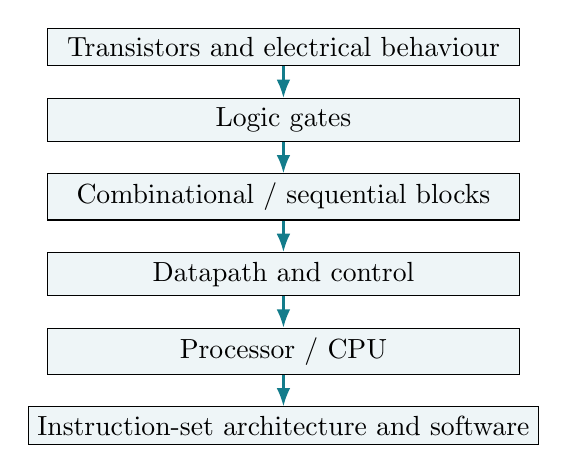
\begin{tikzpicture}[node distance=4mm,>=Latex]\node[draw,fill=pale,minimum width=6cm] (a) {Transistors and electrical behaviour};\node[draw,fill=pale,minimum width=6cm,below=of a] (b) {Logic gates};\node[draw,fill=pale,minimum width=6cm,below=of b] (c) {Combinational / sequential blocks};\node[draw,fill=pale,minimum width=6cm,below=of c] (d) {Datapath and control};\node[draw,fill=pale,minimum width=6cm,below=of d] (e) {Processor / CPU};\node[draw,fill=pale,minimum width=6cm,below=of e] (f) {Instruction-set architecture and software};\foreach \x/\y in {a/b,b/c,c/d,d/e,e/f}{\draw[->,thick,teal](\x)--(\y);}\end{tikzpicture}\end{center}
An unsigned binary number has value $\sum_{i=0}^{n-1}b_i2^i$. Hexadecimal digits represent groups of four bits. Example: $101101_2=45_{10}=2D_{16}$. Two's-complement signed $n$-bit integers range from $-2^{n-1}$ to $2^{n-1}-1$. Carry out and signed overflow are distinct conditions.
\section{Logic gates and Boolean algebra}
NOT inverts, AND is high only when all inputs are high, OR is high when at least one input is high, and XOR is high when inputs differ. NAND and NOR are functionally complete.
\begin{center}\begin{tabular}{cc|ccccc}\toprule $A$&$B$&AND&OR&XOR&NAND&NOR\\\midrule 0&0&0&0&0&1&1\\0&1&0&1&1&1&0\\1&0&0&1&1&1&0\\1&1&1&1&0&0&0\\\bottomrule\end{tabular}\end{center}
\begin{formulaBox}
Identity: $A+0=A$, $A\cdot1=A$. Domination: $A+1=1$, $A\cdot0=0$. Complement: $A+A'=1$, $AA'=0$.\par
De Morgan: $(AB)'=A'+B'$ and $(A+B)'=A'B'$.
\end{formulaBox}
Here $+$ means OR, juxtaposition means AND, and apostrophe means NOT. For $F=AB+AB'$, factor $A$: $F=A(B+B')=A$.
\section{Canonical forms and K-maps}
A truth table specifies every output for every input combination. A minterm is an AND term containing each variable once and is 1 on exactly one row. A maxterm is an OR term containing each variable once and is 0 on exactly one row. Canonical SOP ORs minterms for output-1 rows; canonical POS ANDs maxterms for output-0 rows.
For $F(A,B)=1$ on rows 01 and 10, $F=A'B+AB'=A\oplus B$.
\begin{center}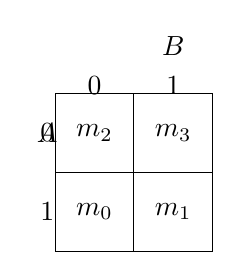
\begin{tikzpicture}[scale=1.0]\node at (1.5,2.6) {$B$};\node at (-.1,1.5) {$A$};\foreach \x/\lab in {0/0,1/1}{\node at (\x+.5,2.1) {\lab};}\foreach \y/\lab in {1/0,0/1}{\node at (-.1,\y+.5) {\lab};}\draw (0,0) grid (2,2);\node at (.5,1.5){$m_2$};\node at (1.5,1.5){$m_3$};\node at (.5,.5){$m_0$};\node at (1.5,.5){$m_1$};\end{tikzpicture}\end{center}
K-map cells use Gray-code ordering so adjacent cells differ in one variable. Group required 1-cells in power-of-two rectangles; edge wrapping and overlapping are permitted when they simplify the expression. Do not include a required zero; use don't-cares only when specification allows.
\section{Timing diagrams and delay}
Propagation delay means the time between an input transition and a corresponding output response. Rise/fall time measures transition speed; glitches are short unintended transitions from unequal path delays. Setup and hold specify data stability windows around a storage element's sampling edge.
\begin{center}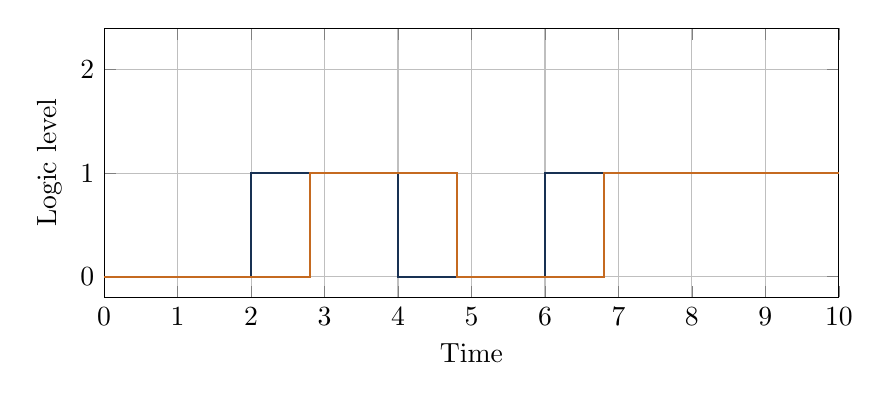
\begin{tikzpicture}\begin{axis}[width=.9\linewidth,height=5cm,xlabel={Time},ylabel={Logic level},xmin=0,xmax=10,ymin=-.2,ymax=2.4,ytick={0,1,2},yticklabels={0,1,2},grid=major]
\addplot[navy,thick,const plot] coordinates {(0,0)(2,1)(4,0)(6,1)(10,1)};
\addplot[orange,thick,const plot] coordinates {(0,0)(2.8,1)(4.8,0)(6.8,1)(10,1)};
\end{axis}\end{tikzpicture}\end{center}
The timing sketch shows an input (navy) and a delayed response (orange). It is conceptual rather than a gate-library timing specification.
\section{Comparators, multiplexers, encoders and decoders}
A one-bit comparator has $A>B=AB'$, $A<B=A'B$, and $A=B=A\operatorname{XNOR}B$. Multi-bit unsigned comparison begins at the most significant bit; the first differing bit determines the outcome.
A 2-to-1 multiplexer selects $D_0$ when $S=0$ and $D_1$ when $S=1$:
\[Y=S'D_0+SD_1.\]
\begin{center}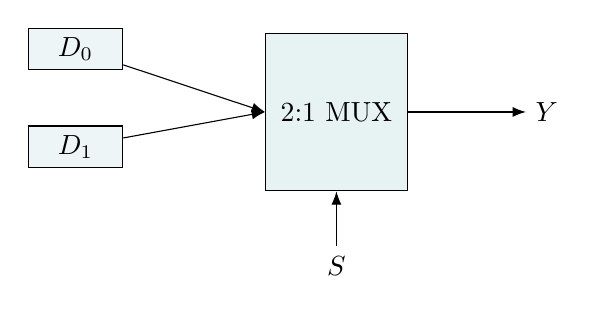
\begin{tikzpicture}[>=Latex,node distance=7mm]\node[draw,fill=pale,minimum width=12mm] (d0) {$D_0$};\node[draw,fill=pale,minimum width=12mm,below=of d0] (d1) {$D_1$};\node[draw,fill=teal!10,minimum width=18mm,minimum height=20mm,right=18mm of d0,yshift=-8mm] (mux) {2:1 MUX};\node[right=15mm of mux] (y) {$Y$};\node[below=of mux] (s) {$S$};\draw[->](d0)--(mux.west);\draw[->](d1)--(mux.west);\draw[->](mux)--(y);\draw[->](s)--(mux.south);\end{tikzpicture}\end{center}
A decoder activates one output for an input code; an encoder maps an active input line to a binary code. A simple encoder assumes only one input active; a priority encoder defines behaviour when several are active.
\section{Adders and arithmetic circuits}
A half adder computes $S=A\oplus B$ and $C=AB$. A full adder includes carry-in: $S=A\oplus B\oplus C_{in}$ and $C_{out}=AB+AC_{in}+BC_{in}$. Ripple carry passes each stage's carry to the next, so worst-case delay tends to rise with width.
\begin{center}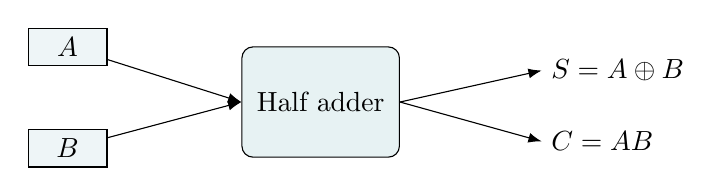
\begin{tikzpicture}[>=Latex,node distance=8mm]\node[draw,fill=pale,minimum width=10mm] (a) {$A$};\node[draw,fill=pale,minimum width=10mm,below=of a] (b) {$B$};\node[draw,rounded corners,fill=teal!10,minimum width=20mm,minimum height=14mm,right=17mm of a,yshift=-7mm] (ha) {Half adder};\node[right=18mm of ha,yshift=4mm] (s) {$S=A\oplus B$};\node[right=18mm of ha,yshift=-5mm] (c) {$C=AB$};\draw[->](a)--(ha.west);\draw[->](b)--(ha.west);\draw[->](ha.east)--(s.west);\draw[->](ha.east)--(c.west);\end{tikzpicture}\end{center}
A PLA has a programmable AND plane for product terms and an OR plane for combining those terms; shared products may reduce hardware cost.
\section{Sequential logic, registers and counters}
Combinational logic maps present inputs to outputs. Sequential logic stores state. A latch is level-sensitive; a flip-flop is edge-triggered. For a D flip-flop, $Q_{next}=D$ at the active edge when timing constraints are met. Violating setup or hold can result in incorrect capture or metastability.
\begin{center}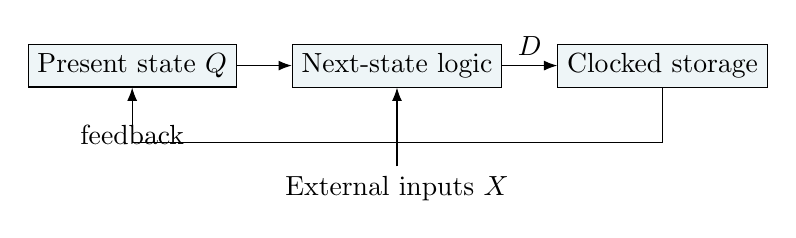
\begin{tikzpicture}[>=Latex,node distance=7mm]\node[draw,fill=pale] (q) {Present state $Q$};\node[draw,fill=pale,right=of q] (logic) {Next-state logic};\node[draw,fill=pale,right=of logic] (ff) {Clocked storage};\draw[->](q)--(logic);\draw[->](logic)--node[above]{$D$}(ff);\draw[->](ff.south) |- ++(0,-.7) -| node[pos=.75,below]{feedback} (q.south);\node[below=10mm of logic] (x) {External inputs $X$};\draw[->](x)--(logic);\end{tikzpicture}\end{center}
A register is a group of flip-flops storing a word. A binary $n$-bit up-counter cycles from 0 through $2^n-1$ and wraps under modulo-$2^n$ operation. A modulo-$N$ counter needs at least $\lceil\log_2N\rceil$ state bits.
\begin{center}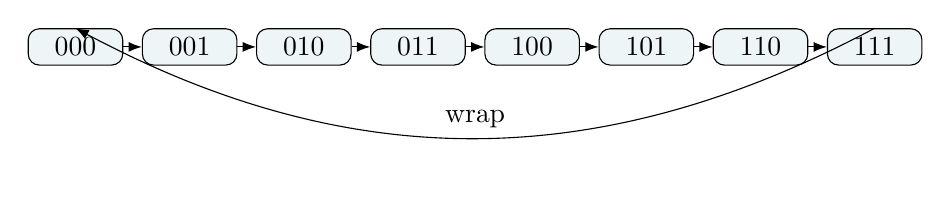
\begin{tikzpicture}[>=Latex]\foreach \i/\v in {0/000,1/001,2/010,3/011,4/100,5/101,6/110,7/111}{\node[draw,rounded corners,fill=pale,minimum width=12mm] (s\i) at (\i*1.45,0) {\v};}\foreach \i in {0,...,6}{\pgfmathtruncatemacro{\j}{\i+1}\draw[->](s\i)--(s\j);}\draw[->,bend left=28] (s7.north) to node[above]{wrap} (s0.north);\end{tikzpicture}\end{center}
\section{Finite-state machines}
An FSM consists of finite states, inputs, a transition function, and outputs. Moore outputs depend on current state; Mealy outputs depend on current state and current inputs.
\topicflow{\node (a) {Describe behaviour};\node (b) [below=of a] {Define states and outputs};\node (c) [below=of b] {Draw state diagram and transition table};\node (d) [below=of c] {Assign codes and derive equations};\node (e) [below=of d] {Implement registers and combinational logic};\node (f) [below=of e] {Simulate transitions, reset and edge cases};\draw (a)--(b);\draw (b)--(c);\draw (c)--(d);\draw (d)--(e);\draw (e)--(f);}
Specify reset state, default transitions, priority when inputs coincide, and behaviour for unused states. Missing transitions or ambiguous input priority make a design underspecified.
\section{Instruction-set architecture (ISA)}
The ISA is the programmer-visible contract: instructions, registers, data types, addressing, memory semantics, exceptions, and control flow. Microarchitecture is the internal design that implements the contract.
\begin{center}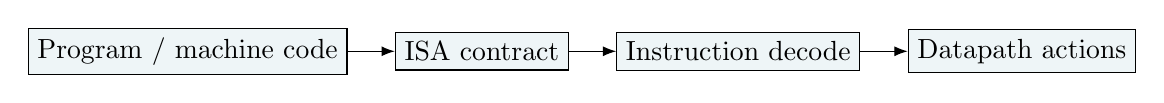
\begin{tikzpicture}[>=Latex,node distance=6mm]\node[draw,fill=pale] (a) {Program / machine code};\node[draw,fill=pale,right=of a] (b) {ISA contract};\node[draw,fill=pale,right=of b] (c) {Instruction decode};\node[draw,fill=pale,right=of c] (d) {Datapath actions};\draw[->](a)--(b);\draw[->](b)--(c);\draw[->](c)--(d);\end{tikzpicture}\end{center}
Conceptually, instruction execution includes fetch, decode, operand read, execute, optional memory access, write-back, and PC update. Single-cycle, multi-cycle, and pipelined implementations organise this differently.
\section{Arithmetic logic unit (ALU)}
An ALU performs addition, subtraction, Boolean operations, shifts, and comparisons. Two's-complement subtraction is often implemented as $A-B=A+\overline{B}+1$. Carry is primarily an unsigned arithmetic condition; signed overflow indicates that the signed mathematical result exceeds the representable range. Status flags and their definitions depend on the ISA.
\begin{center}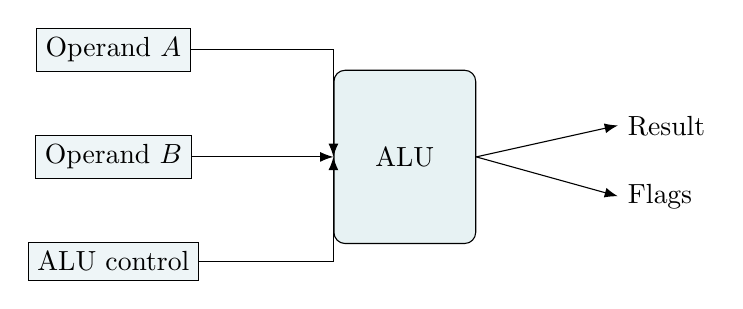
\begin{tikzpicture}[>=Latex,node distance=8mm]\node[draw,fill=pale] (a) {Operand $A$};\node[draw,fill=pale,below=of a] (b) {Operand $B$};\node[draw,fill=pale,below=of b] (c) {ALU control};\node[draw,rounded corners,fill=teal!10,minimum width=18mm,minimum height=22mm,right=18mm of b] (u) {ALU};\node[right=18mm of u,yshift=4mm] (r) {Result};\node[right=18mm of u,yshift=-5mm] (f) {Flags};\draw[->](a.east)-|(u.west);\draw[->](b)--(u.west);\draw[->](c.east)-|(u.west);\draw[->](u.east)--(r.west);\draw[->](u.east)--(f.west);\end{tikzpicture}\end{center}
\section{CPU datapath and control integration}
A basic CPU integrates a program counter and next-PC logic, instruction memory, decoder/control unit, register file, operand multiplexers, ALU, data-memory interface, and write-back selection. Control signals specify register writes, ALU operation, operand selection, memory accesses, write-back source, and PC choice.
\begin{center}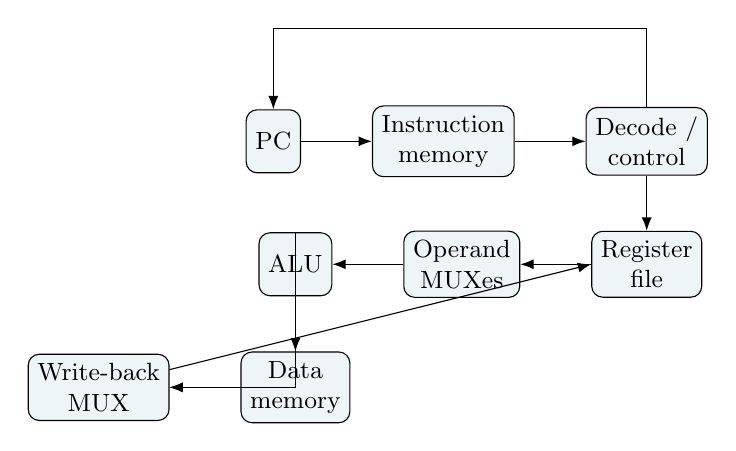
\begin{tikzpicture}[>=Latex,node distance=7mm and 9mm,every node/.style={draw,rounded corners,fill=pale,align=center,font=\small,minimum height=8mm}]\node (pc) {PC};\node (im) [right=of pc] {Instruction\\memory};\node (dec) [right=of im] {Decode /\\control};\node (rf) [below=of dec] {Register\\file};\node (mux) [left=of rf] {Operand\\MUXes};\node (alu) [left=of mux] {ALU};\node (dm) [below=of alu] {Data\\memory};\node (wb) [left=of dm] {Write-back\\MUX};\draw[->](pc)--(im);\draw[->](im)--(dec);\draw[->](dec)--(rf);\draw[->](rf)--(mux);\draw[->](mux)--(alu);\draw[->](alu)--(dm);\draw[->](alu.north) |- (wb.east);\draw[->](dm)--(wb);\draw[->](wb)--(rf.west);\draw[->](dec.north) |- ++(0,1) -| (pc.north);\end{tikzpicture}\end{center}
Single-cycle CPUs complete an instruction in one long cycle; multi-cycle designs reuse hardware across shorter cycles; pipelined CPUs overlap instructions across stages but require hazard handling and more complex control.
\section{Design verification and exam checklist}
\begin{itemize}
\item Build a complete truth table or transition table.
\item Mark active-low signals explicitly and preserve select-bit order.
\item Verify K-map adjacency and every required output-one cell.
\item Check propagation delay, setup, hold, reset and state transitions.
\item Define opcode behaviour and verify ALU flags independently.
\item Trace PC, source operands, ALU result, memory effect, and destination write for each instruction.
\item Test edge cases and undefined/unused state behaviour against the spec.
\end{itemize}
\section{Practice questions}
\begin{enumerate}
\item Simplify $AB+AB'$. \textbf{Answer:} $A(B+B')=A$.
\item When is $A\oplus B=1$? \textbf{Answer:} Inputs differ (01 or 10).
\item For $Y=S'D_0+SD_1$, what is $Y$ when $S=1$? \textbf{Answer:} $D_1$.
\item Half adder when $A=B=1$? \textbf{Answer:} Sum $0$, carry $1$.
\item Minimum bits for 10 states? \textbf{Answer:} $\lceil\log_2 10\rceil=4$.
\item Moore versus Mealy? \textbf{Answer:} Moore output depends on state; Mealy output depends on state and input.
\item ISA versus microarchitecture? \textbf{Answer:} Contract versus its internal implementation.
\end{enumerate}
\section{Source and scope}
Source: \href{https://app.notion.com/p/403a8fc810f681798376c08924a7ca1b}{Computer Systems Design -- Complete Study Notes and Visual Revision Guide}; official outline: \url{https://study.iitm.ac.in/ds/course_pages/BSCS3031.html}. This note set uses general digital-logic and computer-architecture models, not a specification of a particular CPU or ISA. Confirm course-specific simulator conventions and assessment requirements in the live course portal.
\end{document}
